\documentclass[sigconf]{acmart}

% \setcopyright{acmcopyright}
% \copyrightyear{2018}
% \acmYear{2018}
% \acmDOI{XXXXXXX.XXXXXXX}

%% These commands are for a PROCEEDINGS abstract or paper.
% \acmConference[Conference acronym 'XX]{Make sure to enter the correct
%   conference title from your rights confirmation emai}{June 03--05,
%   2018}{Woodstock, NY}
%%
%%  Uncomment \acmBooktitle if the title of the proceedings is different
%%  from ``Proceedings of ...''!
%%
%%\acmBooktitle{Woodstock '18: ACM Symposium on Neural Gaze Detection,
%%  June 03--05, 2018, Woodstock, NY}
% \acmISBN{978-1-4503-XXXX-X/18/06}


%%
%% Submission ID.
%% Use this when submitting an article to a sponsored event. You'll
%% receive a unique submission ID from the organizers
%% of the event, and this ID should be used as the parameter to this command.
%%\acmSubmissionID{123-A56-BU3}


\begin{document}

%%
%% The "title" command has an optional parameter,
%% allowing the author to define a "short title" to be used in page headers.
\title{UnVeilify: A Path Towards Personalized Face Mask Removal}

%%
%% The "author" command and its associated commands are used to define
%% the authors and their affiliations.
%% Of note is the shared affiliation of the first two authors, and the
%% "authornote" and "authornotemark" commands
%% used to denote shared contribution to the research.
\author{Jin Hyoung Joo}
\email{hyoungjoo.j@gmail.com}
\affiliation{%
    \institution{Sungkyunkwan University}
    \country{Republic of South Korea}
}

\author{Minji Kim}
\email{kmjj7864@g.skku.edu}
\affiliation{%
    \institution{Sungkyunkwan University}
    \country{Republic of South Korea}
}

\author{Seungmin Lee}
\email{skghgus9@skku.edu}
\affiliation{%
    \institution{Sungkyunkwan University}
    \country{Republic of South Korea}
}

\author{Hyeonmin Lee}
\email{hyuni7185@g.skku.edu }
\affiliation{%
    \institution{Sungkyunkwan University}
    \country{Republic of South Korea}
}

\author{Hohyun Na}
\email{skghgus9@g.skku.edu}
\affiliation{%
    \institution{Sungkyunkwan University}
    \country{Republic of South Korea}
}

\author{Jaemin You}
\email{yjm7455@g.skku.edu}
\affiliation{%
    \institution{Sungkyunkwan University}
    \country{Republic of South Korea}
}

\begin{abstract}
    Facial masks have been part of many people's lives and therefore a large
    amount of images contain identities wearing these face masks. Our project
    aims to successfully remove these occlusions while retaining the features
    of the target identity. Previous methods of removing facial masks exist,
    however do not consider the importance of identity preservation. We introduce
    a novel neural network architecture that combines the U-Net architecture with
    the StyleGAN generator to achieve this goal.
\end{abstract}

%%
%% The code below is generated by the tool at http://dl.acm.org/ccs.cfm.
%% Please copy and paste the code instead of the example below.
%%
\begin{CCSXML}
<ccs2012>
<concept>
<concept_id>10010147.10010178.10010224.10010245.10010254</concept_id>
<concept_desc>Computing methodologies~Reconstruction</concept_desc>
<concept_significance>300</concept_significance>
</concept>
</ccs2012>
\end{CCSXML}

\ccsdesc[300]{Computing methodologies~Reconstruction}

%%
%% Keywords. The author(s) should pick words that accurately describe
%% the work being presented. Separate the keywords with commas.
\keywords{Generative Adversarial Networks, Personalized Image Generation, Mask Removal, Facial Inpainting,
Facial Reconstruction, Image-to-image Translation}
%% A "teaser" image appears between the author and affiliation
%% information and the body of the document, and typically spans the
%% page.

%%
%% This command processes the author and affiliation and title
%% information and builds the first part of the formatted document.
\maketitle

\section{Introduction}

\section{Related Work}

\paragraph{Image-to-image Translation} {
    pix2pix
}

\paragraph{Generative Adversarial Networks}{
GANs.
}

\section{Method}

Our goal is to remove artifacts covering the facial area, namely face masks,
while preserving the identity of the original person behind the mask. This
requires us to generate the facial features by utilizing some sort of identity
information extracted from an image that contain no occlusions.

Therefore, we obtain two input images from the user, one as the image containing
the face mask to remove (we call this the \emph{masked image}) and the other as
the \emph{identity image} that shows the facial features of the identity the
user wishes to reconstruct. Here, the identity image isn't constrained to any
conditions, \emph{i.e.} the identity image and masked image are expected to be
independent in every way except for the identity of the person.

We first describe the overall architecture that implements the extracted identity features as well as the objective function used in training this model. We then show the identity extraction process.


\subsection{Overall Architecture}
Figure 1 shows the overall architecture of the proposed network, named as \emph{UnVeilify}. The input
masked image goes through an encoder-decoder network, where the decoder is the StyleGAN generator
\cite{StyleGAN}. Although the architecture of this decoder is different in some ways from the
original StyleGAN model, to reduce confusion we leave the name as it is. Further description of this
updated generator architecture can be seen in the following sections.

\begin{figure}[h]
  \centering
  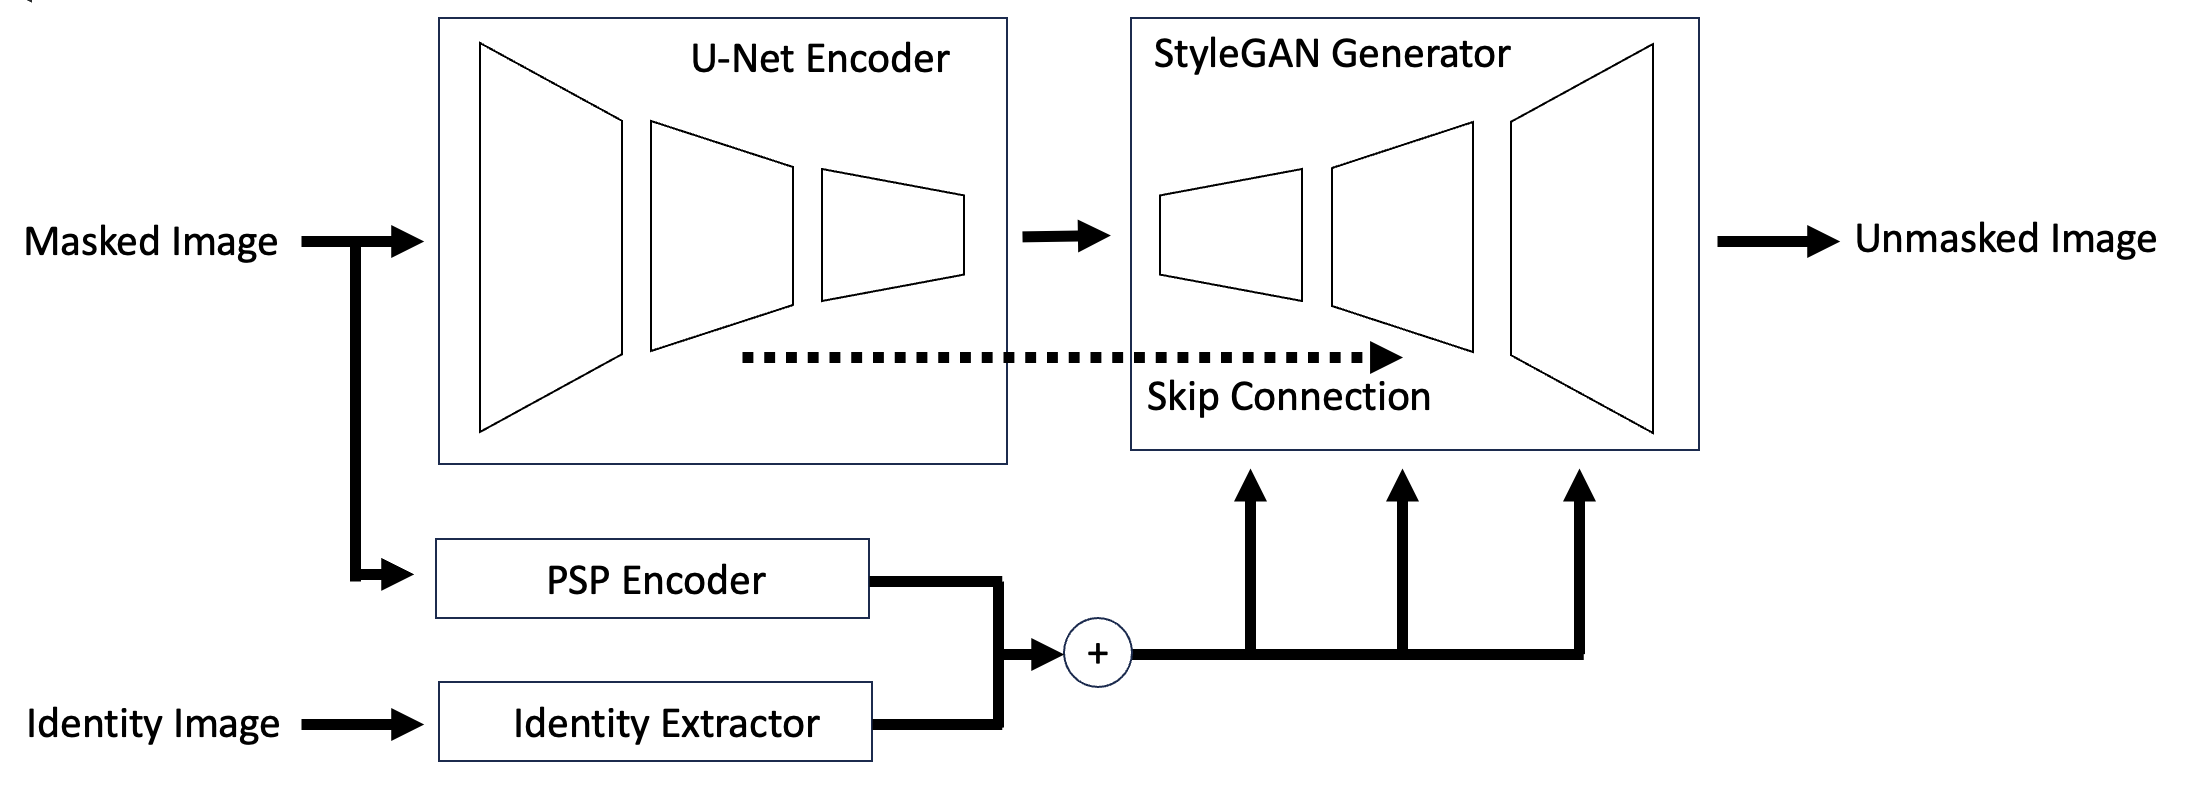
\includegraphics[width=\linewidth]{images/model-architecture.png}
  \caption{TODO: The figure is wrong. Overall architecture of the UnVeilify model.}
  \Description{Overall architecture of the UnVeilify model.}
\end{figure}


\subsection{Identity Extraction}
We use the identity information as the style latent vector that gets projected 
into the StyleGAN generator. Therefore the style vector, denoted as $w$ should be
either $w\in\mathbb{R}^{d}$ or $w\in\mathbb{R}^{L\times d}$. Here, $d$ denotes the
dimension of the latent vector and $L$ denotes the number of layers in the StyleGAN
generator. Due to the higher ability to represent information, we choose to use the
latter, hence the identity image is projected upon the $\mathit{W}^{+}$ latent space.

While there are other possibilites of extracting the identity information, we have
build and conducted experiments only on the following architecture. The encoder we use
is the pixel2style2pixel encoder (pSp encoder) \cite{PSP}. While the details of this
encoder will not be included in this report, the main essence of this encoder is to use
a hierarchial feature pyramid network to extract information from multiple different resolutions
of the image.

Also, while the authors of \cite{PSP} utilized a pretrained StyleGAN generator, due to our
novel network architecture where the original input image features are intact, there is no
need for any pretrained networks. This can help with further expandability to other domains,
especially where specialized datasets are difficult to obtain, since our network can train 
within a end-to-end setting. 

\subsection{Objective Function}
Our models uses several loss functions to achieve the best quality possible. The final
objective function follows the form similar to the objective functions of other image-to-image
translation models.
We first use the $L1$ reconstruction loss in order to generate less blurry images
compared to that of using the $L2$ loss \cite{L1, Pix2Pix}. This loss is used as a
guide for generation by penalizing the distance between the ground truth unmasked image and
generated unmasked image.
\[
    L_{reconstruction}(\mathbf{y}, \mathbf{\hat{y}}) = \|\mathbf{y} - \mathbf{\hat{y}}\|_1
\]

We also use a perceptual loss in order to generate images with high visual qualities. We
utilize the LPIPS loss \cite{LPIPS} in the same way as \cite{PSP} has done,
since it has been shown that the LPIPS
loss preserves image quality better than other perceptual losses \cite{LPIPS2}.
\[
    L_{perceptual}(\mathbf{y}, \mathbf{\hat{y}}) = \|F(\mathbf{y}) - F(\mathbf{\hat{y}})\|_2
\]
Here, $F$ is the feature extractor used for the perceptual loss calculation.

This task focuses highly on identity preservation, where a large portion of the network
architecture design process is shifted towards this specific goal. Hence, in the objective
function we needed a method to also enforce identity preservation. This is achieved by
introducing an identity loss. By taking the cosine similiarity between the features of
a pretrained face recognition network (here we use ArcFace \cite{Arcface}), we can assume
that if the network trains to reduce this loss then the identity information loss would be
minimized.
\[
    L_{identity}(\mathbf{y}, \mathbf{\hat{y}}) = 1- C(R(\mathbf{y}) - R(\mathbf{\hat{y}}))
\]
Here, $R$ is the face recognition backbone model and $C$ is the cosine similiarity
function.

This model follows the form of a generative adversarial network, and incorporates a discriminator
and GAN loss. We use the objective function of the original GAN without any modifications.
However, since the identity image is given as a form of a conditional image, we give the
identity image paired with the unmasked image to the discriminator.
The discriminator is a simple PatchGAN \cite{PatchGAN} discriminator.
\[
    L_{GAN} (G, D) = \mathbb{E}_{y, c}\left[\log D(y, c)\right] + \mathbb{E}_{\hat{y}, c}\left[\log D(\hat{y}, c)\right]
\]

Finally, we use a regularization loss for the facial features in order to normalize
the latent style vectors. This follows the idea of the trucation trick introduced in
StyleGAN.
\[
    L_{reg}(\mathbf{x}) = \|E(\mathbf{x}) - \bar{\mathbf{w}}\|_2
\]

The total objective function is the combination of these 5 separate objective functions.

\section{Experiments}

\section{Conclusion}

\bibliographystyle{ACM-Reference-Format}
\bibliography{citations}



% \subsection{Template Styles}

% The primary parameter given to the ``\verb|acmart|'' document class is
% the {\itshape template style} which corresponds to the kind of publication
% or SIG publishing the work. This parameter is enclosed in square
% brackets and is a part of the {\verb|documentclass|} command:
% \begin{verbatim}
%   \documentclass[STYLE]{acmart}
% \end{verbatim}

% Journals use one of three template styles. All but three ACM journals
% use the {\verb|acmsmall|} template style:
% \begin{itemize}
% \item {\texttt{acmsmall}}: The default journal template style.
% \item {\texttt{acmlarge}}: Used by JOCCH and TAP.
% \item {\texttt{acmtog}}: Used by TOG.
% \end{itemize}

% The majority of conference proceedings documentation will use the {\verb|acmconf|} template style.
% \begin{itemize}
% \item {\texttt{acmconf}}: The default proceedings template style.
% \item{\texttt{sigchi}}: Used for SIGCHI conference articles.
% \item{\texttt{sigplan}}: Used for SIGPLAN conference articles.
% \end{itemize}

% \subsection{Template Parameters}

% In addition to specifying the {\itshape template style} to be used in
% formatting your work, there are a number of {\itshape template parameters}
% which modify some part of the applied template style. A complete list
% of these parameters can be found in the {\itshape \LaTeX\ User's Guide.}

% Frequently-used parameters, or combinations of parameters, include:
% \begin{itemize}
% \item {\texttt{anonymous,review}}: Suitable for a ``double-anonymous''
%   conference submission. Anonymizes the work and includes line
%   numbers. Use with the \texttt{\acmSubmissionID} command to print the
%   submission's unique ID on each page of the work.
% \item{\texttt{authorversion}}: Produces a version of the work suitable
%   for posting by the author.
% \item{\texttt{screen}}: Produces colored hyperlinks.
% \end{itemize}

% This document uses the following string as the first command in the
% source file:
% \begin{verbatim}
% \documentclass[sigconf]{acmart}
% \end{verbatim}

% \section{Modifications}

% Modifying the template --- including but not limited to: adjusting
% margins, typeface sizes, line spacing, paragraph and list definitions,
% and the use of the \verb|\vspace| command to manually adjust the
% vertical spacing between elements of your work --- is not allowed.

% {\bfseries Your document will be returned to you for revision if
%   modifications are discovered.}

% \section{Typefaces}

% The ``\verb|acmart|'' document class requires the use of the
% ``Libertine'' typeface family. Your \TeX\ installation should include
% this set of packages. Please do not substitute other typefaces. The
% ``\verb|lmodern|'' and ``\verb|ltimes|'' packages should not be used,
% as they will override the built-in typeface families.


% \section{Rights Information}

% Authors of any work published by ACM will need to complete a rights
% form. Depending on the kind of work, and the rights management choice
% made by the author, this may be copyright transfer, permission,
% license, or an OA (open access) agreement.

% Regardless of the rights management choice, the author will receive a
% copy of the completed rights form once it has been submitted. This
% form contains \LaTeX\ commands that must be copied into the source
% document. When the document source is compiled, these commands and
% their parameters add formatted text to several areas of the final
% document:
% \begin{itemize}
% \item the ``ACM Reference Format'' text on the first page.
% \item the ``rights management'' text on the first page.
% \item the conference information in the page header(s).
% \end{itemize}

% Rights information is unique to the work; if you are preparing several
% works for an event, make sure to use the correct set of commands with
% each of the works.

% The ACM Reference Format text is required for all articles over one
% page in length, and is optional for one-page articles (abstracts).

% \section{CCS Concepts and User-Defined Keywords}

% Two elements of the ``acmart'' document class provide powerful
% taxonomic tools for you to help readers find your work in an online
% search.

% The ACM Computing Classification System ---
% \url{https://www.acm.org/publications/class-2012} --- is a set of
% classifiers and concepts that describe the computing
% discipline. Authors can select entries from this classification
% system, via \url{https://dl.acm.org/ccs/ccs.cfm}, and generate the
% commands to be included in the \LaTeX\ source.

% User-defined keywords are a comma-separated list of words and phrases
% of the authors' choosing, providing a more flexible way of describing
% the research being presented.

% CCS concepts and user-defined keywords are required for for all
% articles over two pages in length, and are optional for one- and
% two-page articles (or abstracts).

% \section{Sectioning Commands}

% Your work should use standard \LaTeX\ sectioning commands:
% \verb|section|, \verb|subsection|, \verb|subsubsection|, and
% \verb|paragraph|. They should be numbered; do not remove the numbering
% from the commands.

% Simulating a sectioning command by setting the first word or words of
% a paragraph in boldface or italicized text is {\bfseries not allowed.}

% \section{Tables}

% The ``\verb|acmart|'' document class includes the ``\verb|booktabs|''
% package --- \url{https://ctan.org/pkg/booktabs} --- for preparing
% high-quality tables.

% Table captions are placed {\itshape above} the table.

% Because tables cannot be split across pages, the best placement for
% them is typically the top of the page nearest their initial cite.  To
% ensure this proper ``floating'' placement of tables, use the
% environment \textbf{table} to enclose the table's contents and the
% table caption.  The contents of the table itself must go in the
% \textbf{tabular} environment, to be aligned properly in rows and
% columns, with the desired horizontal and vertical rules.  Again,
% detailed instructions on \textbf{tabular} material are found in the
% \textit{\LaTeX\ User's Guide}.

% Immediately following this sentence is the point at which
% Table~\ref{tab:freq} is included in the input file; compare the
% placement of the table here with the table in the printed output of
% this document.

% \begin{table}
%   \caption{Frequency of Special Characters}
%   \label{tab:freq}
%   \begin{tabular}{ccl}
%     \toprule
%     Non-English or Math&Frequency&Comments\\
%     \midrule
%     \O & 1 in 1,000& For Swedish names\\
%     $\pi$ & 1 in 5& Common in math\\
%     \$ & 4 in 5 & Used in business\\
%     $\Psi^2_1$ & 1 in 40,000& Unexplained usage\\
%   \bottomrule
% \end{tabular}
% \end{table}

% To set a wider table, which takes up the whole width of the page's
% live area, use the environment \textbf{table*} to enclose the table's
% contents and the table caption.  As with a single-column table, this
% wide table will ``float'' to a location deemed more
% desirable. Immediately following this sentence is the point at which
% Table~\ref{tab:commands} is included in the input file; again, it is
% instructive to compare the placement of the table here with the table
% in the printed output of this document.

% \begin{table*}
%   \caption{Some Typical Commands}
%   \label{tab:commands}
%   \begin{tabular}{ccl}
%     \toprule
%     Command &A Number & Comments\\
%     \midrule
%     \texttt{{\char'134}author} & 100& Author \\
%     \texttt{{\char'134}table}& 300 & For tables\\
%     \texttt{{\char'134}table*}& 400& For wider tables\\
%     \bottomrule
%   \end{tabular}
% \end{table*}

% Always use midrule to separate table header rows from data rows, and
% use it only for this purpose. This enables assistive technologies to
% recognise table headers and support their users in navigating tables
% more easily.

% \section{Math Equations}
% You may want to display math equations in three distinct styles:
% inline, numbered or non-numbered display.  Each of the three are
% discussed in the next sections.

% \subsection{Inline (In-text) Equations}
% A formula that appears in the running text is called an inline or
% in-text formula.  It is produced by the \textbf{math} environment,
% which can be invoked with the usual
% \texttt{{\char'134}begin\,\ldots{\char'134}end} construction or with
% the short form \texttt{\$\,\ldots\$}. You can use any of the symbols
% and structures, from $\alpha$ to $\omega$, available in
% \LaTeX~\cite{Lamport:LaTeX}; this section will simply show a few
% examples of in-text equations in context. Notice how this equation:
% \begin{math}
%   \lim_{n\rightarrow \infty}x=0
% \end{math},
% set here in in-line math style, looks slightly different when
% set in display style.  (See next section).

% \subsection{Display Equations}
% A numbered display equation---one set off by vertical space from the
% text and centered horizontally---is produced by the \textbf{equation}
% environment. An unnumbered display equation is produced by the
% \textbf{displaymath} environment.

% Again, in either environment, you can use any of the symbols and
% structures available in \LaTeX\@; this section will just give a couple
% of examples of display equations in context.  First, consider the
% equation, shown as an inline equation above:
% \begin{equation}
%   \lim_{n\rightarrow \infty}x=0
% \end{equation}
% Notice how it is formatted somewhat differently in
% the \textbf{displaymath}
% environment.  Now, we'll enter an unnumbered equation:
% \begin{displaymath}
%   \sum_{i=0}^{\infty} x + 1
% \end{displaymath}
% and follow it with another numbered equation:
% \begin{equation}
%   \sum_{i=0}^{\infty}x_i=\int_{0}^{\pi+2} f
% \end{equation}
% just to demonstrate \LaTeX's able handling of numbering.





% \subsection{The ``Teaser Figure''}

% A ``teaser figure'' is an image, or set of images in one figure, that
% are placed after all author and affiliation information, and before
% the body of the article, spanning the page. If you wish to have such a
% figure in your article, place the command immediately before the
% \verb|\maketitle| command:
% \begin{verbatim}
%   \begin{teaserfigure}
%     \includegraphics[width=\textwidth]{sampleteaser}
%     \caption{figure caption}
%     \Description{figure description}
%   \end{teaserfigure}
% \end{verbatim}



% \section{Acknowledgments}

% Identification of funding sources and other support, and thanks to
% individuals and groups that assisted in the research and the
% preparation of the work should be included in an acknowledgment
% section, which is placed just before the reference section in your
% document.

% This section has a special environment:
% \begin{verbatim}
%   \begin{acks}
%   ...
%   \end{acks}
% \end{verbatim}
% so that the information contained therein can be more easily collected
% during the article metadata extraction phase, and to ensure
% consistency in the spelling of the section heading.

% Authors should not prepare this section as a numbered or unnumbered {\verb|\section|}; please use the ``{\verb|acks|}'' environment.

% \section{Appendices}

% If your work needs an appendix, add it before the
% ``\verb|\end{document}|'' command at the conclusion of your source
% document.

% Start the appendix with the ``\verb|appendix|'' command:
% \begin{verbatim}
%   \appendix
% \end{verbatim}
% and note that in the appendix, sections are lettered, not
% numbered. This document has two appendices, demonstrating the section
% and subsection identification method.


% \section{SIGCHI Extended Abstracts}

% The ``\verb|sigchi-a|'' template style (available only in \LaTeX\ and
% not in Word) produces a landscape-orientation formatted article, with
% a wide left margin. Three environments are available for use with the
% ``\verb|sigchi-a|'' template style, and produce formatted output in
% the margin:
% \begin{description}
% \item[\texttt{sidebar}:]  Place formatted text in the margin.
% \item[\texttt{marginfigure}:] Place a figure in the margin.
% \item[\texttt{margintable}:] Place a table in the margin.
% \end{description}

% %%
% %% The acknowledgments section is defined using the "acks" environment
% %% (and NOT an unnumbered section). This ensures the proper
% %% identification of the section in the article metadata, and the
% %% consistent spelling of the heading.
% \begin{acks}
% To Robert, for the bagels and explaining CMYK and color spaces.
% \end{acks}


% %%
% %% If your work has an appendix, this is the place to put it.
% \appendix


\end{document}
\endinput
